\documentclass[]{article}
\usepackage{lmodern}
\usepackage{amssymb,amsmath}
\usepackage{ifxetex,ifluatex}
\usepackage{fixltx2e} % provides \textsubscript
\ifnum 0\ifxetex 1\fi\ifluatex 1\fi=0 % if pdftex
  \usepackage[T1]{fontenc}
  \usepackage[utf8]{inputenc}
\else % if luatex or xelatex
  \ifxetex
    \usepackage{mathspec}
  \else
    \usepackage{fontspec}
  \fi
  \defaultfontfeatures{Ligatures=TeX,Scale=MatchLowercase}
\fi
% use upquote if available, for straight quotes in verbatim environments
\IfFileExists{upquote.sty}{\usepackage{upquote}}{}
% use microtype if available
\IfFileExists{microtype.sty}{%
\usepackage{microtype}
\UseMicrotypeSet[protrusion]{basicmath} % disable protrusion for tt fonts
}{}
\usepackage[margin=1in]{geometry}
\usepackage{hyperref}
\hypersetup{unicode=true,
            pdftitle={R: manipulación de datos},
            pdfborder={0 0 0},
            breaklinks=true}
\urlstyle{same}  % don't use monospace font for urls
\usepackage{color}
\usepackage{fancyvrb}
\newcommand{\VerbBar}{|}
\newcommand{\VERB}{\Verb[commandchars=\\\{\}]}
\DefineVerbatimEnvironment{Highlighting}{Verbatim}{commandchars=\\\{\}}
% Add ',fontsize=\small' for more characters per line
\usepackage{framed}
\definecolor{shadecolor}{RGB}{248,248,248}
\newenvironment{Shaded}{\begin{snugshade}}{\end{snugshade}}
\newcommand{\KeywordTok}[1]{\textcolor[rgb]{0.13,0.29,0.53}{\textbf{#1}}}
\newcommand{\DataTypeTok}[1]{\textcolor[rgb]{0.13,0.29,0.53}{#1}}
\newcommand{\DecValTok}[1]{\textcolor[rgb]{0.00,0.00,0.81}{#1}}
\newcommand{\BaseNTok}[1]{\textcolor[rgb]{0.00,0.00,0.81}{#1}}
\newcommand{\FloatTok}[1]{\textcolor[rgb]{0.00,0.00,0.81}{#1}}
\newcommand{\ConstantTok}[1]{\textcolor[rgb]{0.00,0.00,0.00}{#1}}
\newcommand{\CharTok}[1]{\textcolor[rgb]{0.31,0.60,0.02}{#1}}
\newcommand{\SpecialCharTok}[1]{\textcolor[rgb]{0.00,0.00,0.00}{#1}}
\newcommand{\StringTok}[1]{\textcolor[rgb]{0.31,0.60,0.02}{#1}}
\newcommand{\VerbatimStringTok}[1]{\textcolor[rgb]{0.31,0.60,0.02}{#1}}
\newcommand{\SpecialStringTok}[1]{\textcolor[rgb]{0.31,0.60,0.02}{#1}}
\newcommand{\ImportTok}[1]{#1}
\newcommand{\CommentTok}[1]{\textcolor[rgb]{0.56,0.35,0.01}{\textit{#1}}}
\newcommand{\DocumentationTok}[1]{\textcolor[rgb]{0.56,0.35,0.01}{\textbf{\textit{#1}}}}
\newcommand{\AnnotationTok}[1]{\textcolor[rgb]{0.56,0.35,0.01}{\textbf{\textit{#1}}}}
\newcommand{\CommentVarTok}[1]{\textcolor[rgb]{0.56,0.35,0.01}{\textbf{\textit{#1}}}}
\newcommand{\OtherTok}[1]{\textcolor[rgb]{0.56,0.35,0.01}{#1}}
\newcommand{\FunctionTok}[1]{\textcolor[rgb]{0.00,0.00,0.00}{#1}}
\newcommand{\VariableTok}[1]{\textcolor[rgb]{0.00,0.00,0.00}{#1}}
\newcommand{\ControlFlowTok}[1]{\textcolor[rgb]{0.13,0.29,0.53}{\textbf{#1}}}
\newcommand{\OperatorTok}[1]{\textcolor[rgb]{0.81,0.36,0.00}{\textbf{#1}}}
\newcommand{\BuiltInTok}[1]{#1}
\newcommand{\ExtensionTok}[1]{#1}
\newcommand{\PreprocessorTok}[1]{\textcolor[rgb]{0.56,0.35,0.01}{\textit{#1}}}
\newcommand{\AttributeTok}[1]{\textcolor[rgb]{0.77,0.63,0.00}{#1}}
\newcommand{\RegionMarkerTok}[1]{#1}
\newcommand{\InformationTok}[1]{\textcolor[rgb]{0.56,0.35,0.01}{\textbf{\textit{#1}}}}
\newcommand{\WarningTok}[1]{\textcolor[rgb]{0.56,0.35,0.01}{\textbf{\textit{#1}}}}
\newcommand{\AlertTok}[1]{\textcolor[rgb]{0.94,0.16,0.16}{#1}}
\newcommand{\ErrorTok}[1]{\textcolor[rgb]{0.64,0.00,0.00}{\textbf{#1}}}
\newcommand{\NormalTok}[1]{#1}
\usepackage{graphicx,grffile}
\makeatletter
\def\maxwidth{\ifdim\Gin@nat@width>\linewidth\linewidth\else\Gin@nat@width\fi}
\def\maxheight{\ifdim\Gin@nat@height>\textheight\textheight\else\Gin@nat@height\fi}
\makeatother
% Scale images if necessary, so that they will not overflow the page
% margins by default, and it is still possible to overwrite the defaults
% using explicit options in \includegraphics[width, height, ...]{}
\setkeys{Gin}{width=\maxwidth,height=\maxheight,keepaspectratio}
\IfFileExists{parskip.sty}{%
\usepackage{parskip}
}{% else
\setlength{\parindent}{0pt}
\setlength{\parskip}{6pt plus 2pt minus 1pt}
}
\setlength{\emergencystretch}{3em}  % prevent overfull lines
\providecommand{\tightlist}{%
  \setlength{\itemsep}{0pt}\setlength{\parskip}{0pt}}
\setcounter{secnumdepth}{0}
% Redefines (sub)paragraphs to behave more like sections
\ifx\paragraph\undefined\else
\let\oldparagraph\paragraph
\renewcommand{\paragraph}[1]{\oldparagraph{#1}\mbox{}}
\fi
\ifx\subparagraph\undefined\else
\let\oldsubparagraph\subparagraph
\renewcommand{\subparagraph}[1]{\oldsubparagraph{#1}\mbox{}}
\fi

%%% Use protect on footnotes to avoid problems with footnotes in titles
\let\rmarkdownfootnote\footnote%
\def\footnote{\protect\rmarkdownfootnote}

%%% Change title format to be more compact
\usepackage{titling}

% Create subtitle command for use in maketitle
\newcommand{\subtitle}[1]{
  \posttitle{
    \begin{center}\large#1\end{center}
    }
}

\setlength{\droptitle}{-2em}
  \title{R: manipulación de datos}
  \pretitle{\vspace{\droptitle}\centering\huge}
  \posttitle{\par}
  \author{}
  \preauthor{}\postauthor{}
  \date{}
  \predate{}\postdate{}

\usepackage[
  backend=biber,
  style=alphabetic,
  sorting=ynt,
  citestyle=authoryear
  ]{biblatex}
\addbibresource{../lit/bib.bib}

\usepackage[utf8]{inputenc}
\usepackage[spanish]{babel}

\usepackage{float}
\usepackage{enumitem}
\newcommand\novspace{\@minipagetrue}

%%%% Frames
\ifxetex
    \makeatletter % undo the wrong changes made by mathspec
    \let\RequirePackage\original@RequirePackage
    \let\usepackage\RequirePackage
    \makeatother
\fi

\usepackage{xcolor}
\usepackage[tikz]{bclogo}
\usepackage[framemethod=tikz]{mdframed}
\usepackage{lipsum}
\usepackage[many]{tcolorbox}

\definecolor{bgblue}{RGB}{245,243,253}
\definecolor{ttblue}{RGB}{91,194,224}
\definecolor{llred}{RGB}{255,228,225}
\definecolor{bbblack}{RGB}{0,0,0}

\mdfdefinestyle{mystyle}{%
  rightline=true,
  innerleftmargin=10,
  innerrightmargin=10,
  outerlinewidth=3pt,
  topline=false,
  rightline=true,
  bottomline=false,
  skipabove=\topsep,
  skipbelow=\topsep
}

\newtcolorbox{curiosidad}[1][]{
  breakable,
  title=#1,
  colback=white,
  colbacktitle=white,
  coltitle=black,
  fonttitle=\bfseries,
  bottomrule=0pt,
  toprule=0pt,
  leftrule=3pt,
  rightrule=3pt,
  titlerule=0pt,
  arc=0pt,
  outer arc=0pt,
  colframe=black,
}

\newtcolorbox{nota}[1][]{
  breakable,
  freelance,
  title=#1,
  colback=white,
  colbacktitle=white,
  coltitle=black,
  fonttitle=\bfseries,
  bottomrule=0pt,
  boxrule=0pt,
  colframe=white,
  overlay unbroken and first={
  \draw[red!75!black,line width=3pt]
    ([xshift=5pt]frame.north west) -- 
    (frame.north west) -- 
    (frame.south west);
  \draw[red!75!black,line width=3pt]
    ([xshift=-5pt]frame.north east) -- 
    (frame.north east) -- 
    (frame.south east);
  },
  overlay unbroken app={
  \draw[red!75!black,line width=3pt,line cap=rect]
    (frame.south west) -- 
    ([xshift=5pt]frame.south west);
  \draw[red!75!black,line width=3pt,line cap=rect]
    (frame.south east) -- 
    ([xshift=-5pt]frame.south east);
  },
  overlay middle and last={
  \draw[red!75!black,line width=3pt]
    (frame.north west) -- 
    (frame.south west);
  \draw[red!75!black,line width=3pt]
    (frame.north east) -- 
    (frame.south east);
  },
  overlay last app={
  \draw[red!75!black,line width=3pt,line cap=rect]
    (frame.south west) --
    ([xshift=5pt]frame.south west);
  \draw[red!75!black,line width=3pt,line cap=rect]
    (frame.south east) --
    ([xshift=-5pt]frame.south east);
  },
}

\begin{document}


\section{Datos limpios}\label{datos-limpios}

Esta sección resume algunas de las funciones existentes para
\textbf{limpiar} datos de distintos formatos a \texttt{R}. En
particular, se utiliza la conceptualización de datos limpios presentada
en \textcite{wickham2014tidy} e implementada en el paquete
\texttt{tidyr} \parencite{tidyr}. En la figura \ref{fig:ciclo2} podemos
ver la etapa del análisis de datos correspondiente.

\begin{figure}[h]
    \centering
    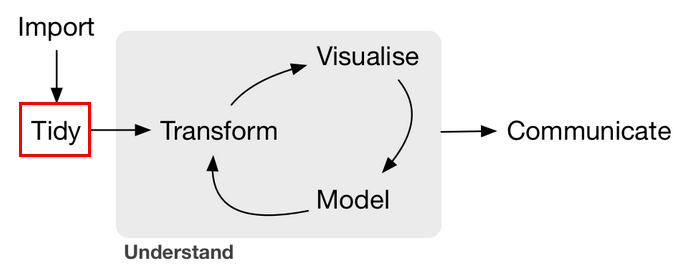
\includegraphics[width=0.75\textwidth]{../img/02_ciclo_2.png}
    \caption{Limpieza de datos \textcite[Introducción]{grolemund2016r}.}
    \label{fig:ciclo2}
\end{figure}

Mucho del esfuerzo en analítica lidia con la limpieza de datos. Tomar
datos de diferentes fuentes y poderlas poner en la forma en la que uno
los necesita para realizar analítica toma mucho tiempo y esfuerzo.
Existen herramientas que permiten que esta parte sea más fácil y
eficiente. Entre éstas se encuentran los criterios de datos limpios.

Los conjuntos de datos limpios (\emph{tidy datasets}) permiten
manipularlos fácilmente, modelarlos y visualizarlos. Aunque funcionan
independientemente del lenguaje utilizado, son particularmente útiles en
\texttt{R} pues éste es un lenguaje pensado para estructuras de datos
tabulares; mismas que son más fácilmente explotables si se usan datos
limpios \parencite{wickham2016r}.

Los datos limpios tienen una estructura específica: cada variable es una
columna, cada observación una fila y tipo de unidad observacional forma
una
tabla\footnote{\textcite[][sección Data Tidying]{wickham2016r} explica este último criterio como ``cada valor ocupa su propia celda''.}.

\subsubsection{Datos limpios en el procesamiento de
datos}\label{datos-limpios-en-el-procesamiento-de-datos}

Esta actividad incluye una gran cantidad de elementos: revisión de
valores atípicos, extracción de variables de cadenas en datos no
estructurados, imputación de valores perdidos. Los datos limpios son tan
solo un subconjunto de este proceso y lidian con el cómo estructurar los
datos de manera que se facilite el análisis.

Los criterios de datos limpios están diseñados para facilitar la
exploración inicial y el análisis de datos, así como simplificar el
desarrollo de herramientas para el análisis de datos que trabajen bien
con datos limpios.

Los criterios de datos limpios están muy relacionados a los de las bases
de datos relacionales y, por ende, al álgebra relacional de Codd
\parencite{wickham2014tidy}. Sin embargo, se expresan y enmarcan en
lenguaje que le es familiar a estadísticos.

Están creados para lidiar con conjuntos de datos que se encuentran en el
mundo real pues -aunque parecen simples- es difícil encontrar datos
limpios de origen. Los criterios de datos limpios proporcionan un marco
mental a través del cual la intuición es explícita, es decir,
proporcionan una manera estándar de ligar la estructura de un dataset
(es decir su layout físico) con su semántica (su significado).

\paragraph{Estructura de datos: un
ejemplo}\label{estructura-de-datos-un-ejemplo}

La mayoría de los datos estadísticos están conformados por tablas
rectangulares compuestas por filas y columnas. Las columnas casi siempre
están etiquetadas (\emph{colnames}) y las filas a veces lo están.

Tomamos el ejemplo de datos de la figura \ref{fig:estructura} en donde
se presentan datos de un
experimento\footnote{Ejemplo tomado de \parencite[][p. 3]{wickham2014tidy}.}.
La tabla contiene dos columnas y tres filas, ambas etiquetadas.

\begin{figure}[h]
    \centering
    \includegraphics[width=0.4\textwidth]{../img/02_estructura.png}
    \caption{Típica presentación de datos.}
    \label{fig:estructura}
\end{figure}

Podemos estructurar los datos de diferentes maneras pero la abstracción
de filas y columnas solamente nos permite pensar en la representación
transpuesta que se muestra en la figura \ref{fig:estructurat}. El diseño
cambia pero los datos son los mismos. Además de la apariencia,
deberíamos de poder describir la semántica -el significado- de los
valores que se muestran en una tabla \parencite[][p. 3]{wickham2014tidy}
pero la abstracción de filas y columnas no da para más.

\begin{figure}[h]
    \centering
    \includegraphics[width=0.5\textwidth]{../img/02_estructurat.png}
    \caption{Mismos datos que en \ref{fig:estructura} pero traspuestos.}
    \label{fig:estructurat}
\end{figure}

\subsubsection{Semántica}\label{semantica}

Un conjunto de datos es una colección de \textbf{valores} (normalmente
cuantitativos/números o cualitativos/caracteres). Los valores se
organizan de dos maneras: cada valor pertenece simultáneamente a una
variable y a una observación.

\begin{itemize}
\tightlist
\item
  Una \emph{variable} contiene todos los valores de una medida y del
  mismo atributo subyacente (por ejemplo, temperatura, duración, altura,
  latitud) a través de unidades.
\item
  Una \emph{observación}, en cambio, contiene todos los valores medidos
  para la misma unidad (por ejemplo, una persona, un día, un municipio)
  a través de distintos atributos.
\end{itemize}

Los mismos datos en las figuras \ref{fig:estructura} y
\ref{fig:estructurat} los pensamos ahora en estos términos. Tenemos 3
variables:

\begin{enumerate}
\def\labelenumi{\arabic{enumi}.}
\tightlist
\item
  \emph{persona} con tres posibles valores (John, Jane, Mary)
\item
  \emph{tratamiento} con dos posibles valores (a o b)
\item
  \emph{resultado} con 6 valores (-, 16, 3, 2, 11, 1)
\end{enumerate}

El diseño del experimento mismo nos habla de la estructura de las
observaciones y los posibles valores que pueden tomar. Por ejemplo, en
este caso el valor perdido nos dice que, por diseño, se debió de
capturar esta variable pero no se hizo (por eso es importante guardarlo
como tal)\footnote{Los valores perdidos estructurales, representan
  mediciones de valores que no se puede hacer o que no suceden y, por
  tanto, se pueden eliminar (por ejemplo, hombres embarazados). En este
  ejemplo, tenemos un valor perdido no estructural.}.

En la figura \ref{fig:estructuratidy} se muestran los mismos datos que
antes pero pensados tal que las variables son columnas y las
observaciones (en este caso, cada punto en el diseño experimental) son
filas.

\begin{figure}[h]
    \centering
    \includegraphics[width=0.4\textwidth]{../img/02_estructuratidy.png}
    \caption{Observaciones son filas, variables columnas.}
    \label{fig:estructuratidy}
\end{figure}

Normalmente, es fácil determinar cuáles son las observaciones y cuáles
son las variables en los distintos casos, pero es difícil dar una
definición en forma precisa. Por ejemplo, si tienes teléfonos de casa y
celulares, se pueden considerar como dos variables distintas en muchos
contextos pero en prevención de fraude necesitas una variable que guarde
el tipo de teléfono y otra en la que se guarde el número pues el uso
regular del mismo número de teléfono por parte de la misma persona puede
ayudar a detectarlo.

En general, es más fácil describir las \emph{relaciones funcionales
entre las variables} que entre las filas pues las puedes operar
fácilmente: por ejemplo, el radio entre dos variables, una combinación
lineal de varias variables. También es más fácil \emph{hacer
comparaciones entre grupos de observaciones} que entre columnas: la
suma, el promedio, la varianza, la moda
\parencite[][p. 4]{wickham2014tidy}.

Las observaciones, por su parte, son más complejas pues normalmente
\emph{se enmarcan en un análisis específico} que se desea realizar con
los datos y existen varios niveles. Por ejemplo, en un análisis de
ingreso podemos tener datos sociodemográficos de los individuos, datos
geográficos del lugar en el que viven, datos macroeconómicos del tiempo
específico, datos de la familia del individuo, datos del trabajo del
individuo, entre otros.

\subsection{Datos limpios}\label{datos-limpios-1}

Éstos mapean de forma estándar el significado y la estructura de los
datos. Un conjunto de datos se considera sucio o limpio dependiendo de
cómo las filas, columnas y tablas mapean a observaciones, variables y
tipos. En \textbf{datos limpios}:

\begin{enumerate}
\def\labelenumi{\arabic{enumi}.}
\tightlist
\item
  Cada \emph{variable} es una columna.
\item
  Cada \emph{observación} es una fila.
\item
  Cada \emph{tipo de unidad observacional} es una tabla / cada valor
  tiene su celda.
\end{enumerate}

En la figura \ref{fig:datoslimpios} podemos ver estos tres elementos de
los datos limpios y cómo se representan en un \emph{dataframe}.

\begin{figure}[h]
    \centering
    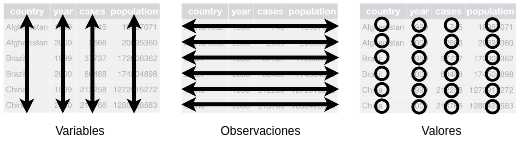
\includegraphics[width=0.9\textwidth]{../img/datos_limpios.png}
    \caption{Ejemplificación de datos limpios \parencite[][sección Data Tidying]{wickham2016r}.}
    \label{fig:datoslimpios}
\end{figure}

Esto equivale a la tercera forma normal de Codd
\parencite[][p. 4]{wickham2014tidy} enfocado a un solo conjunto de datos
y no a datos conectados como en bases relacionales. Los datos sucios son
cualquier otro tipo de manera de organizar los datos.

La tabla \ref{fig:estructuratidy} corresponde a datos limpios: cada fila
es una observación, es decir, el resultado de un tratamiento a una
persona. Cada columna es una variable. Solo tenemos un tipo de unidad
observacional, es decir, cada renglón es una unidad del diseño
experimental.

Con los datos así ordenados, suele ser más fácil extraer datos que, por
ejemplo, en Tabla \ref{fig:estructura}.

\renewcommand\bcStyleTitre[1]{\large\textcolor{bbblack}{#1}}

\begin{bclogo}[
  couleur=llred,
  arrondi=0,
  logo=\bcstop,
  barre=none,
  noborder=true]{Ejercicios}
\begin{enumerate}
\item Crea un dataframe con los valores de la tabla \ref{fig:estructura} y otro 
con los valores de la tabla \ref{fig:estructuratidy}.
\item Extrae el resultado para (John Smith, tratamiento a) en la primera configuración y en la segunda.
\item Especifica el número de tratamientos con la forma sucia y la forma limpia.
\item ¿Cuál es la media de los resultados? Usa la forma 1 y la forma 2.
\item Extrae los tratamientos del tipo a en la forma 2.
\end{enumerate}

\end{bclogo}

Los datos limpios permiten hacerle preguntas a los datos de manera
simple y sistemática. En particular, es una estructura muy útil para
programación vectorizada como la que \texttt{R} tiene (el ejercicio 5)
porque la \emph{forma} en la que almacenamos los datos se asegura que
valores para diferentes variables de la misma observación siempre están
apareados.

Por convención, las variables se acomodan de una forma particular. Las
variables \emph{fijas} (en este ejemplo, las propias al diseño
experimental) van primero y posteriormente las variables \emph{medidas}.
Ordenamos éstas de forma que las que están relacionadas sean contiguas.

\subsection{De sucio a limpio}\label{de-sucio-a-limpio}

Los conjuntos de datos normalmente \textbf{no cumplen} con estos
criterios. Es raro obtener un conjunto de datos con el cuál podemos
trabajar de manera inmediata.

Los 5 problemas más comunes para llevar datos sucios a limpios
\parencite[][p. 5]{wickham2014tidy} son:

\begin{enumerate}
\def\labelenumi{\arabic{enumi}.}
\tightlist
\item
  Los nombres de las columnas son valores, no nombres de variables.
\item
  Múltiples variables se encuentran en la misma columna.
\item
  Las variables están guardadas tanto en filas como en columnas.
\item
  Muchos tipos de unidad observacional se encuentran en la misma tabla.
\item
  Una sola unidad observacional se guardó en varias tablas.
\end{enumerate}

Estos problemas pueden ser resueltos con las funciones implementadas en
el paquete \texttt{tidyr}: \texttt{gather}, \texttt{spread},
\texttt{separate} y \texttt{unite}.

\subsubsection{Los nombres de las columnas son valores, no nombres de
variables}\label{los-nombres-de-las-columnas-son-valores-no-nombres-de-variables}

La tabla \ref{tab:varsencols} muestra datos sucios con este problema. La
base acompaña al paquete \texttt{tidyr} \parencite{tidyr} y es una
muestra de los datos del reporte sobre tuberculosis de la organización
mundial de la salud. Contiene observaciones anuales por país para casos
de tuberculosis según distintos grupos.

La descripción de todas las variables se puede ver tecleando
\texttt{?who}

Dentro de un reporte, la representación que se tiene de las variables
tiene sentido. Por ejemplo, en la tabla \ref{tab:varsencols} vemos los
casos de tuberculosis para distintos grupos de edad de hombres en México
para cierto tipo de diagnóstico.

\begin{table}[H]
\centering
\begingroup\tiny
\begin{tabular}{lrrrrrrrr}
  \hline
country & year & new\_sp\_m014 & new\_sp\_m1524 & new\_sp\_m2534 & new\_sp\_m3544 & new\_sp\_m4554 & new\_sp\_m5564 & new\_sp\_m65 \\ 
  \hline
Mexico & 2000 & 214 & 1079 & 1387 & 1162 & 1235 & 972 & 1126 \\ 
  Mexico & 2001 & 130 & 1448 & 1639 & 1683 & 1606 & 1229 & 1566 \\ 
  Mexico & 2002 & 154 & 1090 & 1292 & 1301 & 1146 & 986 & 1144 \\ 
  Mexico & 2003 & 187 & 1207 & 1461 & 1417 & 1313 & 1005 & 1352 \\ 
  Mexico & 2004 &  86 & 1053 & 1276 & 1181 & 1201 & 958 & 1209 \\ 
  Mexico & 2005 & 100 & 1095 & 1376 & 1314 & 1238 & 1042 & 1288 \\ 
  Mexico & 2006 & 129 & 986 & 1320 & 1333 & 1275 & 1012 & 1215 \\ 
  Mexico & 2007 & 145 & 981 & 1286 & 1286 & 1266 & 942 & 1226 \\ 
  Mexico & 2008 & 124 & 966 & 1292 & 1314 & 1267 & 1004 & 1213 \\ 
  Mexico & 2009 & 103 & 1030 & 1262 & 1401 & 1360 & 1024 & 1252 \\ 
  Mexico & 2010 & 125 & 1081 & 1375 & 1380 & 1392 & 1119 & 1303 \\ 
   \hline
\end{tabular}
\endgroup
\caption{Casos de tuberculosis para México del 2000 al 2010 para hombres con diagnóstico por lesiones de pulmón.} 
\label{tab:varsencols}
\end{table}

En las columnas tenemos varias variables: método de diagnóstico, género
y categorías de edad. Para arreglarlo, necesitamos \emph{juntar}
(gather) las columnas con valores de variables en una sola columna que
contenga esos nombres como valores. En otras palabras, debemos convertir
de la columna 5 en adelante en filas.

Con el paquete \textbf{tidyr} esto se puede realizar en forma fácil con
el comando \texttt{gather} de manera que obtenemos un dataframe como el
que se muestra en la tabla \ref{tab:varsjuntadas}.

\begin{Shaded}
\begin{Highlighting}[]
\NormalTok{junta <-}\StringTok{ }\NormalTok{tidyr}\OperatorTok{::}\KeywordTok{gather}\NormalTok{(who, }\DataTypeTok{key =}\NormalTok{ variables, }\DataTypeTok{value =}\NormalTok{ casos}
\NormalTok{                       , }\OperatorTok{-}\NormalTok{country, }\OperatorTok{-}\NormalTok{iso2, }\OperatorTok{-}\NormalTok{iso3, }\OperatorTok{-}\NormalTok{year, }\DataTypeTok{na.rm =}\NormalTok{ T)}
\end{Highlighting}
\end{Shaded}

Los parámetros que recibe la función gather son (al menos):

\begin{itemize}
\tightlist
\item
  El \emph{data.frame} como primer parámetro.
\item
  La llave (parámetro \emph{key}) será el nombre que tomará la variable
  con los nombres de las columnas a juntar.
\item
  El valor (parámetro \emph{value}) es el nombre de la variable que
  contendrá los valores correspondientes a cada valor (el diagnóstico
  \(i-ésimo\), el \(j-ésimo\) género y el \(k-ésimo\) grupo de edad).
\item
  Al último, especificamos las variables que \textbf{NO} se deben de
  juntar (en este caso: el país, iso2, iso3 y el año).
\end{itemize}

Hay parámetros opcionales en la función. Para estos datos en particular,
por ejemplo, es conveniente remover los grupos para los que no se tiene
el dato con el parámetro \texttt{na.rm\ =\ TRUE}.

\begin{table}[ht]
\centering
\begingroup\tiny
\begin{tabular}{lllrlr}
  \hline
country & iso2 & iso3 & year & variables & casos \\ 
  \hline
Afghanistan & AF & AFG & 1997 & new\_sp\_m014 &   0 \\ 
  Afghanistan & AF & AFG & 1998 & new\_sp\_m014 &  30 \\ 
  Afghanistan & AF & AFG & 1999 & new\_sp\_m014 &   8 \\ 
  Afghanistan & AF & AFG & 2000 & new\_sp\_m014 &  52 \\ 
  Afghanistan & AF & AFG & 2001 & new\_sp\_m014 & 129 \\ 
  Afghanistan & AF & AFG & 2002 & new\_sp\_m014 &  90 \\ 
   \hline
\end{tabular}
\endgroup
\caption{Valores de variables en una sola variable.} 
\label{tab:varsjuntadas}
\end{table}

\begin{nota} 
\textbf{gather\\}

En la figura se ejemplifica la operacionalización de `gather` para los datos de tratamiento.

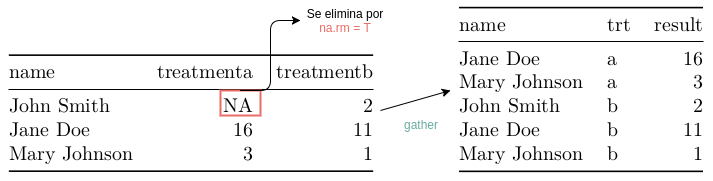
\includegraphics[width=0.9\textwidth]{../img/gather.png}

Esto es resultado de ejecutar: \\

\begin{verbatim}
gather(fig1, key = trt, value = result, -name, na.rm = T) %>% 
  mutate(trt = gsub("treatment", "", trt))
\end{verbatim}

\end{nota}

\renewcommand\bcStyleTitre[1]{\large\textcolor{bbblack}{#1}}

\begin{bclogo}[
  couleur=llred,
  arrondi=0,
  logo=\bcstop,
  barre=none,
  noborder=true]{Ejercicio}

Este tipo de formato de datos (poner valores de variables en las columnas) 
es útil también cuando se capturan datos al evitar la repetición de valores. \\

Por ejemplo, pensemos en un experimento clínico en el que seguimos a sujetos
a lo largo de un tratamiento midiendo su IMC. Una forma muy
sencilla de guardar los datos del experimento es utilizando un procesador
de texto común. El capturista no querrá seguir criterios de datos limpios
al llenar la información pues implicaría repetir el nombre de la persona,
el día de la captura y el nivel de colesterol. Supongamos un experimento con
16 sujetos a lo largo de un año en donde se mide el colesterol una vez al mes (mes1, mes2, etc.). Los datos capturados se muestran en la tabla \ref{tab:sujetos}. \\

Nuevamente, queremos convertir la columna 3 a 14 en filas, es decir, observaciones.
Utiliza el comando `gather` para realizar esto y obtener el resultado que se
muestra en la tabla \ref{tab:sujetostidy}.
\end{bclogo}

\begin{table}[H]
\centering
\begingroup\tiny
\begin{tabular}{llrrrrrrrrrrrr}
  \hline
sujetos & grupo & mes1 & mes2 & mes3 & mes4 & mes5 & mes6 & mes7 & mes8 & mes9 & mes10 & mes11 & mes12 \\ 
  \hline
A & control & 23.46 & 24.86 & 25.25 & 25.18 & 25.79 & 25.90 & 26.02 & 26.24 & 27.85 & 27.55 & 28.07 & 27.39 \\ 
  B & tratamiento & 22.73 & 23.33 & 25.44 & 26.10 & 24.85 & 25.36 & 25.70 & 25.55 & 26.77 & 28.43 & 28.26 & 28.93 \\ 
  C & control & 26.80 & 26.95 & 27.47 & 27.11 & 28.56 & 29.35 & 29.74 & 31.04 & 32.37 & 32.37 & 33.18 & 32.19 \\ 
  D & control & 31.08 & 31.72 & 31.04 & 30.58 & 31.92 & 33.24 & 32.06 & 31.29 & 31.55 & 30.36 & 30.72 & 30.89 \\ 
  E & control & 19.07 & 17.65 & 17.30 & 17.14 & 17.11 & 17.39 & 19.11 & 19.12 & 18.64 & 18.73 & 19.92 & 19.87 \\ 
  F & control & 19.18 & 18.81 & 20.20 & 21.24 & 22.82 & 24.50 & 25.23 & 26.09 & 24.97 & 26.37 & 28.18 & 28.18 \\ 
  G & tratamiento & 33.53 & 32.79 & 32.94 & 33.87 & 34.82 & 34.82 & 34.87 & 33.97 & 34.18 & 34.78 & 33.68 & 35.36 \\ 
  H & tratamiento & 20.20 & 21.11 & 23.15 & 24.67 & 24.33 & 26.24 & 27.57 & 27.88 & 29.70 & 31.76 & 31.98 & 31.53 \\ 
  I & control & 19.84 & 21.73 & 20.98 & 22.12 & 22.24 & 23.73 & 24.22 & 23.08 & 21.84 & 22.43 & 22.60 & 23.06 \\ 
  J & tratamiento & 25.08 & 25.08 & 25.35 & 26.13 & 27.71 & 28.61 & 27.93 & 26.91 & 27.51 & 27.41 & 27.87 & 27.35 \\ 
  K & control & 19.76 & 20.98 & 20.09 & 21.90 & 21.73 & 23.54 & 25.66 & 26.40 & 27.47 & 26.41 & 28.22 & 30.77 \\ 
  L & control & 25.11 & 26.30 & 25.56 & 27.17 & 29.32 & 29.47 & 29.34 & 31.59 & 32.60 & 32.85 & 33.01 & 33.24 \\ 
  M & control & 33.69 & 34.61 & 36.90 & 36.51 & 36.56 & 36.98 & 38.92 & 40.26 & 42.56 & 42.68 & 43.35 & 43.52 \\ 
  N & control & 28.18 & 27.48 & 28.46 & 28.91 & 30.38 & 29.29 & 29.06 & 29.68 & 31.65 & 31.95 & 33.92 & 33.72 \\ 
  O & control & 31.94 & 31.74 & 31.73 & 31.69 & 33.14 & 32.84 & 31.13 & 30.93 & 31.11 & 30.49 & 31.10 & 32.80 \\ 
  P & control & 17.99 & 18.08 & 15.83 & 16.70 & 19.22 & 19.39 & 20.94 & 20.87 & 20.20 & 19.98 & 19.92 & 20.65 \\ 
   \hline
\end{tabular}
\endgroup
\caption{Mediciones de IMC en sujetos.} 
\label{tab:sujetos}
\end{table}

\begin{table}[H]
\centering
\begin{tabular}{lllr}
  \hline
sujetos & grupo & mes & IMC \\ 
  \hline
D & control & mes9 & 31.55 \\ 
  K & control & mes1 & 19.76 \\ 
  G & tratamiento & mes6 & 34.82 \\ 
  E & control & mes10 & 18.73 \\ 
  C & control & mes12 & 32.19 \\ 
  H & tratamiento & mes3 & 23.15 \\ 
  O & control & mes5 & 33.14 \\ 
  M & control & mes10 & 42.68 \\ 
  B & tratamiento & mes3 & 25.44 \\ 
  L & control & mes8 & 31.59 \\ 
   \hline
\end{tabular}
\caption{Muestra de datos limpios para experimentos IMC.} 
\label{tab:sujetostidy}
\end{table}

\begin{Shaded}
\begin{Highlighting}[]
\CommentTok{# Creamos los datos}
\NormalTok{df <-}\StringTok{ }\KeywordTok{data.frame}\NormalTok{(}
  \DataTypeTok{sujetos =}\NormalTok{ LETTERS[}\DecValTok{1}\OperatorTok{:}\DecValTok{16}\NormalTok{],}
  \DataTypeTok{grupo =} \KeywordTok{sample}\NormalTok{(}\KeywordTok{c}\NormalTok{(}\StringTok{"control"}\NormalTok{, }\StringTok{"tratamiento"}\NormalTok{), }\DataTypeTok{size =} \DecValTok{16}\NormalTok{, }\DataTypeTok{replace =}\NormalTok{ T, }\DataTypeTok{prob =} \KeywordTok{c}\NormalTok{(}\FloatTok{0.5}\NormalTok{, }\FloatTok{0.5}\NormalTok{))}
  \CommentTok{# ,  meses = as.vector(sapply(paste0("mes",1:12), rep, 16))}
\NormalTok{  )}
\NormalTok{m <-}\StringTok{ }\KeywordTok{t}\NormalTok{(}\KeywordTok{sapply}\NormalTok{(}\KeywordTok{runif}\NormalTok{(}\DecValTok{16}\NormalTok{, }\DecValTok{16}\NormalTok{, }\DecValTok{35}\NormalTok{), }\DataTypeTok{FUN =} \ControlFlowTok{function}\NormalTok{(x)\{}\KeywordTok{cumsum}\NormalTok{(}\KeywordTok{c}\NormalTok{(x, }\KeywordTok{rnorm}\NormalTok{(}\DecValTok{11}\NormalTok{, }\DataTypeTok{mean =} \FloatTok{0.5}\NormalTok{, }\DataTypeTok{sd =} \DecValTok{1}\NormalTok{)))\}))}
\KeywordTok{colnames}\NormalTok{(m) <-}\StringTok{ }\KeywordTok{paste0}\NormalTok{(}\StringTok{"mes"}\NormalTok{,}\DecValTok{1}\OperatorTok{:}\DecValTok{12}\NormalTok{)}
\NormalTok{df <-}\StringTok{ }\KeywordTok{cbind}\NormalTok{(df, m)}

\CommentTok{# Respuesta: opción 1}
\NormalTok{tidyr}\OperatorTok{::}\KeywordTok{gather}\NormalTok{(df, }\DataTypeTok{key =}\NormalTok{ mes, }\DataTypeTok{value =}\NormalTok{ IMC, }\OperatorTok{-}\NormalTok{sujetos, }\OperatorTok{-}\NormalTok{grupo)}
\CommentTok{# opción 2}
\NormalTok{tidyr}\OperatorTok{::}\KeywordTok{gather}\NormalTok{(df, }\DataTypeTok{key =}\NormalTok{ mes, }\DataTypeTok{value =}\NormalTok{ IMC, mes1}\OperatorTok{:}\NormalTok{mes12)}
\end{Highlighting}
\end{Shaded}

\subsubsection{Múltiples variables se encuentran en la misma
columna}\label{multiples-variables-se-encuentran-en-la-misma-columna}

Otra forma de datos sucios es cuando una columna con nombres de
variables tiene realmente varias variables dentro del nombre.

Si regresamos al ejemplo de la sección anterior, podemos notar que
todavía no se tienen datos limpios. Primero, notamos una redundancia:
todos los valores tienen el sufijo ``new\_'' o ``new'' pero éste no
tiene significado. Eliminamos ese pedazo de texto de los valores con la
función \texttt{gsub}.

Segundo, debemos extraer los valores de las variables método de
diagnóstico, género y categoría de edad de la columna que acabamos de
construir (que llamamos ``variables'').

En la descripción de las variables (teclea \texttt{?who}) se describen a
los títulos de las columnas (que ahora están guardados en la variable
\emph{variables}) tales que contienen como prefijo ``new\_'', seguido
del diagnóstico que puede ser de dos o tres caracteres, ``\_f" para
mujeres o ``\_m" para hombres y, por último, el rango de edad.

\begin{curiosidad}[Expresiones regulares o regex]
En esencia, las \textit{regex} (por el inglés regular expressions) utilizan 
caracteres para definir patrones de más caracteres. Éstos se conocen como 
metacaracteres y pueden ser herramientas poderosas en la limpieza de datos.

Pueden ser utilizadas para buscar una cadena en específico en forma exacta, 
buscar una cadena dentro de otra o para reemplazar una parte de una cadena con
otra cosa.

\textcite[][sección ``text processing and regular expressions'']{peng2016m} 
realiza una buena revisión de las funciones disponibles en \texttt{R} para 
utilizar expresiones regulares. 
\end{curiosidad}

Para eso, utilizamos la función \texttt{extract} del paquete
\texttt{tidyr}. A esta función, debemos decirle cuál es el nombre de la
variable que contiene varios valores (parámetro \emph{col}), los nuevos
nombres de columnas (parámetro \emph{into}) y la expresión regular con
la que irá capturando los pedazos y asignándolos a la columna correcta
(parámetro \emph{regex}).

\begin{Shaded}
\begin{Highlighting}[]
\NormalTok{limpios <-}\StringTok{ }\NormalTok{junta }\OperatorTok
\StringTok{  }\KeywordTok{mutate}\NormalTok{(}\DataTypeTok{variables =} \KeywordTok{gsub}\NormalTok{(}\StringTok{"new_|new"}\NormalTok{, }\StringTok{""}\NormalTok{, variables)) }\OperatorTok
\StringTok{  }\NormalTok{tidyr}\OperatorTok{::}\KeywordTok{extract}\NormalTok{(., }\DataTypeTok{col =}\NormalTok{ variables}
\NormalTok{          , }\DataTypeTok{into =} \KeywordTok{c}\NormalTok{(}\StringTok{"diagnostico"}\NormalTok{, }\StringTok{"genero"}\NormalTok{, }\StringTok{"edad"}\NormalTok{)}
\NormalTok{          , }\DataTypeTok{regex =} \StringTok{"([[:alnum:]]+)_([a-z])([[0-9]]+)"}\NormalTok{) }
\end{Highlighting}
\end{Shaded}

Por último, se deben limpiar las categorías de edad. En este caso, se
decide volverlos un factor con las categorías ordenadas por los grupos
de edad existentes en la base:

\begin{Shaded}
\begin{Highlighting}[]
\NormalTok{limpios }\OperatorTok
\StringTok{  }\KeywordTok{mutate}\NormalTok{(}
    \DataTypeTok{edad =} \KeywordTok{factor}\NormalTok{(edad, }
                  \DataTypeTok{levels =} \KeywordTok{c}\NormalTok{(}\StringTok{"014"}\NormalTok{, }\StringTok{"1524"}\NormalTok{, }\StringTok{"2534"}\NormalTok{, }\StringTok{"3544"}
\NormalTok{                             , }\StringTok{"4554"}\NormalTok{, }\StringTok{"5564"}\NormalTok{, }\StringTok{"65"}\NormalTok{)}
\NormalTok{                  , }\DataTypeTok{labels =} \KeywordTok{c}\NormalTok{(}\StringTok{"0-14"}\NormalTok{, }\StringTok{"15-24"}\NormalTok{, }\StringTok{"25-34"}\NormalTok{, }\StringTok{"35-44"}
\NormalTok{                               , }\StringTok{"45-54"}\NormalTok{, }\StringTok{"55-64"}\NormalTok{, }\StringTok{"65>"}\NormalTok{)}
\NormalTok{                  , }\DataTypeTok{ordered =}\NormalTok{ T)}
\NormalTok{  )}
\end{Highlighting}
\end{Shaded}

\begin{nota}[Nota]
Nota como en el último ejemplo, se utiliza el símbolo \texttt{\%$<>$\%} que es 
equivalente a realizar una asignación ($<-$) y un pipe (\texttt{\%$>$\%}) de los datos 
que están guardados en el dataframe limpios.
\end{nota}

De esta forma, obtenemos los datos como se ven en la tabla
\ref{tab:varslimpios} donde tenemos una variable para el método de
diagnóstico, una para el género, otra para la edad y una última con el
número de casos observados.

\begin{table}[ht]
\centering
\begingroup\tiny
\begin{tabular}{lllrlllr}
  \hline
country & iso2 & iso3 & year & diagnostico & genero & edad & casos \\ 
  \hline
Afghanistan & AF & AFG & 1997 & sp & m & 0-14 &   0 \\ 
  Afghanistan & AF & AFG & 1998 & sp & m & 0-14 &  30 \\ 
  Afghanistan & AF & AFG & 1999 & sp & m & 0-14 &   8 \\ 
  Afghanistan & AF & AFG & 2000 & sp & m & 0-14 &  52 \\ 
  Afghanistan & AF & AFG & 2001 & sp & m & 0-14 & 129 \\ 
  Afghanistan & AF & AFG & 2002 & sp & m & 0-14 &  90 \\ 
   \hline
\end{tabular}
\endgroup
\caption{Cada columna es una variable.} 
\label{tab:varslimpios}
\end{table}

\begin{nota}[Nota] 
Esta forma es limpia pues cada columna es una variable, cada fila es una observación
y no se mezclan unidades observacionales.
\end{nota}

\renewcommand\bcStyleTitre[1]{\large\textcolor{bbblack}{#1}}

\begin{bclogo}[
  couleur=llred,
  arrondi=0,
  logo=\bcstop,
  barre=none,
  noborder=true]{Ejercicio}
  
A continuación se crea el dataframe \textit{pob} que contiene un identificador
para el individuo (id) y una columna llamada \textit{variables} que contiene
el sexo, año de nacimiento y la altura en centímetros todos en una columna y
separados por ``\_''. \\

Utiliza la función \texttt{separate} del paquete \texttt{tidyr} para limpiar
estos datos.
\end{bclogo}

\begin{Shaded}
\begin{Highlighting}[]
\CommentTok{# Respuestas}
\CommentTok{# Generamos los datos}
\NormalTok{pob <-}\StringTok{ }\KeywordTok{tibble}\NormalTok{(}
  \DataTypeTok{id =} \DecValTok{1}\OperatorTok{:}\DecValTok{1000}
\NormalTok{  , }\DataTypeTok{variables =} \KeywordTok{paste0}\NormalTok{(}
    \KeywordTok{sample}\NormalTok{(}\DataTypeTok{x =} \KeywordTok{c}\NormalTok{(}\StringTok{'f'}\NormalTok{, }\StringTok{'m'}\NormalTok{), }\DataTypeTok{size =} \DecValTok{1000}\NormalTok{, }\DataTypeTok{replace =}\NormalTok{ T)}
\NormalTok{    , }\StringTok{"_"}
\NormalTok{    , }\KeywordTok{floor}\NormalTok{(}\KeywordTok{runif}\NormalTok{(}\DecValTok{1000}\NormalTok{, }\DecValTok{45}\NormalTok{, }\DecValTok{99}\NormalTok{))}
\NormalTok{    , }\StringTok{"_"}
\NormalTok{    , }\KeywordTok{floor}\NormalTok{(}\KeywordTok{runif}\NormalTok{(}\DecValTok{1000}\NormalTok{, }\DecValTok{50}\NormalTok{, }\DecValTok{190}\NormalTok{))}
\NormalTok{  )}
\NormalTok{)}

\CommentTok{# Utilizamos separate para generar las variables:}
\CommentTok{# sexo, año de nacimiento y altura}
\NormalTok{pob.tidy <-}\StringTok{ }\NormalTok{pob }\OperatorTok
\StringTok{  }\KeywordTok{separate}\NormalTok{(}\DataTypeTok{col =}\NormalTok{ variables}
\NormalTok{           , }\DataTypeTok{into =} \KeywordTok{c}\NormalTok{(}\StringTok{"sexo"}\NormalTok{, }\StringTok{"anio_nac"}\NormalTok{, }\StringTok{"altura"}\NormalTok{), }\DataTypeTok{sep =} \StringTok{"_"}\NormalTok{)}

\CommentTok{# Pasamos a enteros las variables anio de nac y altura}
\NormalTok{pob.tidy }\OperatorTok
\StringTok{  }\KeywordTok{mutate_each}\NormalTok{(}\KeywordTok{funs}\NormalTok{(as.integer), anio_nac, altura)}

\NormalTok{pob.tidy}
\end{Highlighting}
\end{Shaded}

\subsubsection{Las variables están guardadas tanto en filas como en
columnas}\label{las-variables-estan-guardadas-tanto-en-filas-como-en-columnas}

Uno de los problemas más difíciles es cuando las variables están tanto
en filas como en columnas.

Para ejemplificar este problema, se muestran los datos de temperatura
máxima y mínima en algunas zonas de México
\parencite[][archivo: data/weather.txt]{tidydata}. Los datos que
limpiaremos se ven en la tabla \ref{tab:clima}. Como se puede ver,
tenemos valores del día del mes de la observación como nombres de
variables: d1 (día 1), d2 (día 2), etc. Esto es homólogo al problema 1
visto anteriormente.

También tenemos variables en las filas: la temperatura máxima y la
temperatura mínima deberían ser el nombre de las columnas.

\begin{table}[ht]
\centering
\begingroup\tiny
\begin{tabular}{lrrlrrrrrrrrrrr}
  \hline
id & year & month & element & d1 & d2 & d3 & d4 & d5 & d6 & d7 & d8 & d9 & d10 & d11 \\ 
  \hline
MX17004 & 2010 &   1 & tmax &  &  &  &  &  &  &  &  &  &  &  \\ 
  MX17004 & 2010 &   1 & tmin &  &  &  &  &  &  &  &  &  &  &  \\ 
  MX17004 & 2010 &   2 & tmax &  & 27.30 & 24.10 &  &  &  &  &  &  &  & 29.70 \\ 
  MX17004 & 2010 &   2 & tmin &  & 14.40 & 14.40 &  &  &  &  &  &  &  & 13.40 \\ 
  MX17004 & 2010 &   3 & tmax &  &  &  &  & 32.10 &  &  &  &  & 34.50 &  \\ 
  MX17004 & 2010 &   3 & tmin &  &  &  &  & 14.20 &  &  &  &  & 16.80 &  \\ 
  MX17004 & 2010 &   4 & tmax &  &  &  &  &  &  &  &  &  &  &  \\ 
  MX17004 & 2010 &   4 & tmin &  &  &  &  &  &  &  &  &  &  &  \\ 
  MX17004 & 2010 &   5 & tmax &  &  &  &  &  &  &  &  &  &  &  \\ 
  MX17004 & 2010 &   5 & tmin &  &  &  &  &  &  &  &  &  &  &  \\ 
  MX17004 & 2010 &   6 & tmax &  &  &  &  &  &  &  &  &  &  &  \\ 
  MX17004 & 2010 &   6 & tmin &  &  &  &  &  &  &  &  &  &  &  \\ 
  MX17004 & 2010 &   7 & tmax &  &  & 28.60 &  &  &  &  &  &  &  &  \\ 
  MX17004 & 2010 &   7 & tmin &  &  & 17.50 &  &  &  &  &  &  &  &  \\ 
  MX17004 & 2010 &   8 & tmax &  &  &  &  & 29.60 &  &  & 29.00 &  &  &  \\ 
  MX17004 & 2010 &   8 & tmin &  &  &  &  & 15.80 &  &  & 17.30 &  &  &  \\ 
  MX17004 & 2010 &  10 & tmax &  &  &  &  & 27.00 &  & 28.10 &  &  &  &  \\ 
  MX17004 & 2010 &  10 & tmin &  &  &  &  & 14.00 &  & 12.90 &  &  &  &  \\ 
  MX17004 & 2010 &  11 & tmax &  & 31.30 &  & 27.20 & 26.30 &  &  &  &  &  &  \\ 
  MX17004 & 2010 &  11 & tmin &  & 16.30 &  & 12.00 & 7.90 &  &  &  &  &  &  \\ 
  MX17004 & 2010 &  12 & tmax & 29.90 &  &  &  &  & 27.80 &  &  &  &  &  \\ 
  MX17004 & 2010 &  12 & tmin & 13.80 &  &  &  &  & 10.50 &  &  &  &  &  \\ 
   \hline
\end{tabular}
\endgroup
\caption{Mediciones de temperatura max y min.} 
\label{tab:clima}
\end{table}

Para limpiar, lo primero que debemos hacer es juntar los días (que son
valores de la variable día) en una sola columna. Después utilizamos la
nueva variable para crear la fecha. Así, obtenemos la tabla
\ref{tab:clima1}, a partir de los datos en el dataframe \emph{raw}.

\begin{Shaded}
\begin{Highlighting}[]
\CommentTok{# Tidy}
\CommentTok{# Primero, juntamos la variable dias}
\NormalTok{clean1 <-}\StringTok{ }\NormalTok{tidyr}\OperatorTok{::}\KeywordTok{gather}\NormalTok{(raw, }\DataTypeTok{key =}\NormalTok{ variable, }\DataTypeTok{value =}\NormalTok{ value, d1}\OperatorTok{:}\NormalTok{d31}
\NormalTok{                        , }\DataTypeTok{na.rm =}\NormalTok{ T)}

\CommentTok{# Después, generamos la variable día y fecha}
\NormalTok{clean1}\OperatorTok{$}\NormalTok{day <-}\StringTok{ }\KeywordTok{as.integer}\NormalTok{(}\KeywordTok{str_replace}\NormalTok{(clean1}\OperatorTok{$}\NormalTok{variable, }\StringTok{"d"}\NormalTok{, }\StringTok{""}\NormalTok{))}
\NormalTok{clean1}\OperatorTok{$}\NormalTok{date <-}\StringTok{ }\KeywordTok{as.Date}\NormalTok{(}\KeywordTok{ISOdate}\NormalTok{(clean1}\OperatorTok{$}\NormalTok{year, clean1}\OperatorTok{$}\NormalTok{month, clean1}\OperatorTok{$}\NormalTok{day))}

\CommentTok{# Seleccionamos las variables limpias y ordenamos}
\NormalTok{clean1 <-}\StringTok{ }\NormalTok{dplyr}\OperatorTok{::}\KeywordTok{select_}\NormalTok{(clean1, }\StringTok{"id"}\NormalTok{, }\StringTok{"date"}\NormalTok{, }\StringTok{"element"}\NormalTok{, }\StringTok{"value"}\NormalTok{) }\OperatorTok
\StringTok{  }\NormalTok{dplyr}\OperatorTok{::}\KeywordTok{arrange}\NormalTok{(date, element) }
\end{Highlighting}
\end{Shaded}

\begin{nota}[stringr]
Otro paquete muy útil para realizar tareas de limpieza con cadenas. 
La \href{https://cran.r-project.org/web/packages/stringr/stringr.pdf}{documentación}
detalla todas sus funciones. En este caso, utilizamos la función \texttt{str\_replace}
que nos permite reemplazar una cadena de caracteres por otra.
\end{nota}

\begin{table}[ht]
\centering
\begin{tabular}{lrlr}
  \hline
id & date & element & value \\ 
  \hline
MX17004 & 14639.00 & tmax & 27.80 \\ 
  MX17004 & 14639.00 & tmin & 14.50 \\ 
  MX17004 & 14642.00 & tmax & 27.30 \\ 
  MX17004 & 14642.00 & tmin & 14.40 \\ 
  MX17004 & 14643.00 & tmax & 24.10 \\ 
   \hline
\end{tabular}
\caption{Paso 1. Juntar las columnas, limpiar dias, crear fecha.} 
\label{tab:clima1}
\end{table}

El segundo paso es transformar la variable \texttt{element} en dos
columnas pues, en realidad, almacena dos variables: temperatura máxima y
mínima.

\begin{Shaded}
\begin{Highlighting}[]
\CommentTok{# Las temperaturas van a columnas}
\NormalTok{clean2 <-}\StringTok{ }\NormalTok{tidyr}\OperatorTok{::}\KeywordTok{spread}\NormalTok{(clean1, }\DataTypeTok{key =}\NormalTok{ element, }\DataTypeTok{value =}\NormalTok{ value)}
\end{Highlighting}
\end{Shaded}

\begin{table}[ht]
\centering
\begin{tabular}{lrlr}
  \hline
id & date & element & value \\ 
  \hline
MX17004 & 14639.00 & tmax & 27.80 \\ 
  MX17004 & 14639.00 & tmin & 14.50 \\ 
  MX17004 & 14642.00 & tmax & 27.30 \\ 
  MX17004 & 14642.00 & tmin & 14.40 \\ 
  MX17004 & 14643.00 & tmax & 24.10 \\ 
   \hline
\end{tabular}
\caption{Paso 2. Enviar a columnas las mediciones de temperaturas.} 
\label{tab:clima1}
\end{table}

En este caso, se utilizó la función \texttt{spread} del paquete
\texttt{tidyr}. Esta función realiza una especie de inverso a la
operación que hace \texttt{gather}. En lugar de juntar nombres de
variables, utiliza los valores de una variable como nombres de columnas
(parámetro \emph{key}) y rellena apropiadamente las celdas con los
valores de otra variable (parámetro \emph{value}). Los demás parámetros
son opcionales y, por ejemplo, en lugar de tener un parámetro para
especificar qué hacer con los \texttt{NA} (en gather: \texttt{na.rm}),
en este caso pide el parámetro \texttt{fill} cuyo default es \texttt{NA}
pero, en algunos casos, es más apropiado insertar otro valor para
rellenar valores de celdas en donde no había un valor correspondiente.

\subsubsection{Muchos tipos de unidad observacional se encuentran en la
misma
tabla}\label{muchos-tipos-de-unidad-observacional-se-encuentran-en-la-misma-tabla}

En ocasiones las bases de datos involucran diferentes tipos de unidad
observacional. Para tener datos limpios, cada unidad observacional debe
estar almacenada en su propia tabla.

Para este ejemplo, utilizamos la base de datos \texttt{billboard}
\parencite[][archivo: data/billboard.csv]{tidydata}

\begin{Shaded}
\begin{Highlighting}[]
\NormalTok{billboard <-}\StringTok{ }\NormalTok{readr}\OperatorTok{::}\KeywordTok{read_csv}\NormalTok{(}\StringTok{"tidyr_datasets/billboard.csv"}\NormalTok{)}
\NormalTok{billboard_long <-}\StringTok{ }\KeywordTok{gather}\NormalTok{(billboard, week, rank, x1st.week}\OperatorTok{:}\NormalTok{x76th.week}
\NormalTok{                         , }\DataTypeTok{na.rm =} \OtherTok{TRUE}\NormalTok{)}
\NormalTok{billboard_tidy <-}\StringTok{ }\NormalTok{billboard_long }\OperatorTok
\StringTok{  }\KeywordTok{mutate}\NormalTok{(}
    \DataTypeTok{week =} \KeywordTok{extract_numeric}\NormalTok{(week),}
    \DataTypeTok{date =} \KeywordTok{as.Date}\NormalTok{(date.entered) }\OperatorTok{+}\StringTok{ }\DecValTok{7} \OperatorTok{*}\StringTok{ }\NormalTok{(week }\OperatorTok{-}\StringTok{ }\DecValTok{1}\NormalTok{)) }\OperatorTok
\StringTok{    }\KeywordTok{select}\NormalTok{(}\OperatorTok{-}\NormalTok{date.entered)}
\KeywordTok{head}\NormalTok{(billboard_tidy)}
\end{Highlighting}
\end{Shaded}

\begin{verbatim}
## # A tibble: 6 x 9
##    year     artist.inverted                                 track     time
##   <int>               <chr>                                 <chr>   <time>
## 1  2000     Destiny's Child              Independent Women Part I 03:38:00
## 2  2000             Santana                          Maria, Maria 04:18:00
## 3  2000       Savage Garden                    I Knew I Loved You 04:07:00
## 4  2000             Madonna                                 Music 03:45:00
## 5  2000 Aguilera, Christina Come On Over Baby (All I Want Is You) 03:38:00
## 6  2000               Janet                 Doesn't Really Matter 04:17:00
## # ... with 5 more variables: genre <chr>, date.peaked <date>, week <dbl>,
## #   rank <chr>, date <date>
\end{verbatim}

\renewcommand\bcStyleTitre[1]{\large\textcolor{bbblack}{#1}}

\begin{bclogo}[
  couleur=llred,
  arrondi=0,
  logo=\bcstop,
  barre=none,
  noborder=true]{Ejercicio}
  
¿Cuáles son las unidades observacionales en esta tabla?
\end{bclogo}

\begin{Shaded}
\begin{Highlighting}[]
\CommentTok{# Respuesta}

\CommentTok{# Tenemos por un lado una unidad observacional: las características de la}
\CommentTok{# canción.}

\CommentTok{# Por el otro tenemos otra unidad observacional: las posiciones que tuvieron }
\CommentTok{# las canciones en cada semana.}
\end{Highlighting}
\end{Shaded}

Debemos separar las unidades observacionales, esto significa separar la
base de datos en dos: la tabla \emph{canciones} que almacena artista,
nombre de la canción y duración; la tabla \emph{posiciones} que almacena
el ranking de la canción en cada semana.

\begin{Shaded}
\begin{Highlighting}[]
\NormalTok{canciones <-}\StringTok{ }\NormalTok{billboard_tidy }\OperatorTok\StringTok{ }
\StringTok{  }\KeywordTok{select}\NormalTok{(artist.inverted, track, year, time) }\OperatorTok
\StringTok{  }\KeywordTok{unique}\NormalTok{() }\OperatorTok
\StringTok{  }\KeywordTok{arrange}\NormalTok{(artist.inverted) }\OperatorTok
\StringTok{  }\KeywordTok{mutate}\NormalTok{(}\DataTypeTok{song_id =} \KeywordTok{row_number}\NormalTok{(artist.inverted))}

\KeywordTok{head}\NormalTok{(canciones, }\DecValTok{5}\NormalTok{)}
\end{Highlighting}
\end{Shaded}

\begin{verbatim}
## # A tibble: 5 x 5
##   artist.inverted
##             <chr>
## 1           2 Pac
## 2         2Ge+her
## 3    3 Doors Down
## 4    3 Doors Down
## 5        504 Boyz
## # ... with 4 more variables: track <chr>, year <int>, time <time>,
## #   song_id <int>
\end{verbatim}

\begin{Shaded}
\begin{Highlighting}[]
\NormalTok{posiciones <-}\StringTok{ }\NormalTok{billboard_tidy }\OperatorTok
\StringTok{  }\KeywordTok{left_join}\NormalTok{(canciones, }\KeywordTok{c}\NormalTok{(}\StringTok{"artist.inverted"}\NormalTok{, }\StringTok{"track"}\NormalTok{, }\StringTok{"year"}\NormalTok{, }\StringTok{"time"}\NormalTok{)) }\OperatorTok
\StringTok{  }\KeywordTok{select}\NormalTok{(song_id, date, week, rank) }\OperatorTok
\StringTok{  }\KeywordTok{arrange}\NormalTok{(song_id, date) }\OperatorTok
\StringTok{  }\NormalTok{tbl_df}
\NormalTok{posiciones}
\end{Highlighting}
\end{Shaded}

\begin{verbatim}
## # A tibble: 5,307 x 4
##    song_id       date  week  rank
##      <int>     <date> <dbl> <chr>
##  1       1 2000-02-26     1    87
##  2       1 2000-03-04     2    82
##  3       1 2000-03-11     3    72
##  4       1 2000-03-18     4    77
##  5       1 2000-03-25     5    87
##  6       1 2000-04-01     6    94
##  7       1 2000-04-08     7    99
##  8       2 2000-09-02     1    91
##  9       2 2000-09-09     2    87
## 10       2 2000-09-16     3    92
## # ... with 5,297 more rows
\end{verbatim}

\subsubsection{Una sola unidad observarcional se guardó en varias
tablas}\label{una-sola-unidad-observarcional-se-guardo-en-varias-tablas}

Este ejemplo y datos se toman de \textcite{tutorialintro}.

Es común que los valores sobre una misma unidad observacional estén
separados en varios archivos. Muchas veces, cada archivo es una
variable, e.g.~el mes o el nombre del paciente, etc. Para limpiar estos
datos debemos:

\begin{enumerate}
\def\labelenumi{\arabic{enumi}.}
\tightlist
\item
  Leemos los archivos en una lista de tablas.
\item
  Para cada tabla agregamos una columna que registra el nombre del
  archivo original.
\item
  Combinamos las tablas en un solo dataframe.
\end{enumerate}

La carpeta \texttt{tidyr\_datasets/specdata} contiene 332 archivos csv
que almacenan información de monitoreo de contaminación en 332
ubicaciones de EUA. Cada archivo contiene información de una unidad de
monitoreo y el número de identificación del monitor es el nombre del
archivo.

Primero creamos un vector con los nombres de los archivos en un
directorio con extensión .csv.

\begin{Shaded}
\begin{Highlighting}[]
\NormalTok{paths <-}\StringTok{ }\KeywordTok{dir}\NormalTok{(}\StringTok{"tidyr_datasets/specdata"}\NormalTok{, }\DataTypeTok{pattern =} \StringTok{"}\CharTok{\textbackslash{}\textbackslash{}}\StringTok{.csv$"}
\NormalTok{             , }\DataTypeTok{full.names =} \OtherTok{TRUE}\NormalTok{)}
\KeywordTok{names}\NormalTok{(paths) <-}\StringTok{ }\KeywordTok{basename}\NormalTok{(paths)}
\NormalTok{specdata_US <-}\StringTok{ }\KeywordTok{tbl_df}\NormalTok{(}\KeywordTok{ldply}\NormalTok{(paths, read.csv, }\DataTypeTok{stringsAsFactors =} \OtherTok{FALSE}\NormalTok{))}
\NormalTok{specdata_US }\OperatorTok\StringTok{ }\NormalTok{head}
\end{Highlighting}
\end{Shaded}

\begin{verbatim}
## # A tibble: 6 x 5
##       .id       Date sulfate nitrate    ID
##     <chr>      <chr>   <dbl>   <dbl> <int>
## 1 001.csv 2003-01-01      NA      NA     1
## 2 001.csv 2003-01-02      NA      NA     1
## 3 001.csv 2003-01-03      NA      NA     1
## 4 001.csv 2003-01-04      NA      NA     1
## 5 001.csv 2003-01-05      NA      NA     1
## 6 001.csv 2003-01-06      NA      NA     1
\end{verbatim}

Las variables quedaron un poco sucias\ldots{} las limpiamos y
seleccionamos solo las de interés.

\begin{Shaded}
\begin{Highlighting}[]
\NormalTok{specdata <-}\StringTok{ }\NormalTok{specdata_US }\OperatorTok
\StringTok{  }\KeywordTok{mutate}\NormalTok{(}
    \DataTypeTok{monitor =} \KeywordTok{extract_numeric}\NormalTok{(.id),}
    \DataTypeTok{date =} \KeywordTok{as.Date}\NormalTok{(Date)) }\OperatorTok
\StringTok{    }\KeywordTok{select}\NormalTok{(}\DataTypeTok{id =}\NormalTok{ ID, monitor, date, sulfate, nitrate)}
\NormalTok{specdata }\OperatorTok\StringTok{ }\NormalTok{head}
\end{Highlighting}
\end{Shaded}

\begin{verbatim}
## # A tibble: 6 x 5
##      id monitor       date sulfate nitrate
##   <int>   <dbl>     <date>   <dbl>   <dbl>
## 1     1       1 2003-01-01      NA      NA
## 2     1       1 2003-01-02      NA      NA
## 3     1       1 2003-01-03      NA      NA
## 4     1       1 2003-01-04      NA      NA
## 5     1       1 2003-01-05      NA      NA
## 6     1       1 2003-01-06      NA      NA
\end{verbatim}

\renewcommand\bcStyleTitre[1]{\large\textcolor{bbblack}{#1}}

\begin{bclogo}[
  couleur=llred,
  arrondi=0,
  logo=\bcstop,
  barre=none,
  noborder=true]{Ejercicio}

En la carpeta \texttt{tidyr\_datasets\/informe\/} se encuentran dos archivos que
contienen los datos de la relación del pago de pensiones del IMSS e ISSSTE respecto 
a su gasto programable devengado por entidad federativa. 

Los datos tienen todos los problemas explorados en esta sección, salvo el que 
solo hay un tipo de unidad observacional.

Los datos están divididos en los archivos \texttt{M2\_218.xlsx} y 
\texttt{M2\_219.xlsx} y se puede observar un ejemplo de éstos en la figura \ref{fig:ejerciciofinal}.
El ejercicio consiste en leer los datos y limpiarlos de forma que sean datos
limpios\footnote{Los datos fueron tomados de \textcite[][p. 218-219]{informe} y el catálogo de estados se tomó de \parencite{mgn}}.

\end{bclogo}

\begin{figure}[h]
    \centering
    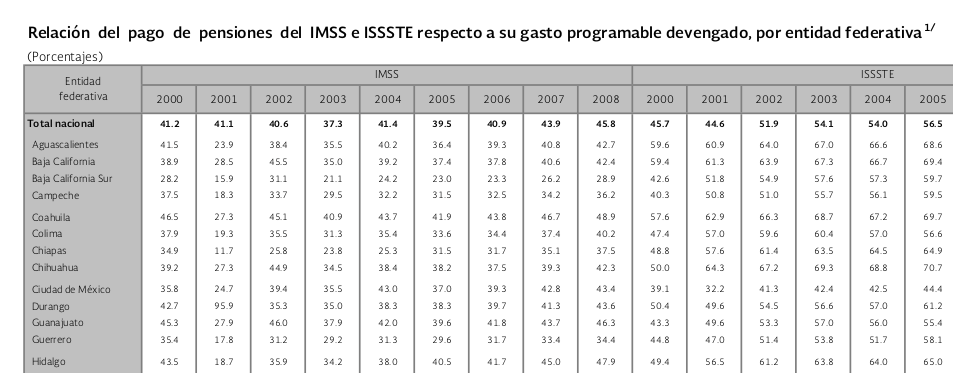
\includegraphics[width=0.75\textwidth]{../img/ejercicio_tidy_informe.png}
    \caption{Datos de pensiones del IMSS e ISSSTE 2000 a 2016 \parencite[][p. 218-219]{informe}.}
    \label{fig:ejerciciofinal}
\end{figure}

\begin{Shaded}
\begin{Highlighting}[]
\CommentTok{# Respuesta}
\KeywordTok{rm}\NormalTok{(}\DataTypeTok{list =} \KeywordTok{ls}\NormalTok{())}
\CommentTok{# Funciones auxiliares}

\CommentTok{# Como son archivos de excel, muchas líneas están vacias pero R no }
\CommentTok{# lo entiende. Esta función quita esas lineas.}
\NormalTok{quita.nas <-}\StringTok{ }\ControlFlowTok{function}\NormalTok{(df, }\DataTypeTok{prop.na =} \FloatTok{0.8}\NormalTok{) \{}
\NormalTok{  df <-}\StringTok{ }\NormalTok{df[, }\OperatorTok{!}\KeywordTok{is.na}\NormalTok{(}\KeywordTok{names}\NormalTok{(df)) }\OperatorTok{&}\StringTok{ }\KeywordTok{names}\NormalTok{(df) }\OperatorTok{!=}\StringTok{ ""}\NormalTok{]}
\NormalTok{  r <-}\StringTok{ }\KeywordTok{sapply}\NormalTok{(}\KeywordTok{seq}\NormalTok{(}\KeywordTok{nrow}\NormalTok{(df)), }\DataTypeTok{FUN =} \ControlFlowTok{function}\NormalTok{(x)\{}
    \KeywordTok{sum}\NormalTok{(}\KeywordTok{is.na}\NormalTok{(df[x,]))}
\NormalTok{  \})}
\NormalTok{  r <-}\StringTok{ }\NormalTok{r}\OperatorTok{/}\KeywordTok{ncol}\NormalTok{(df)}
\NormalTok{  df[r }\OperatorTok{<}\StringTok{ }\NormalTok{prop.na, ]}
\NormalTok{\}}

\CommentTok{# Como pegaremos estados a partir de sus nombres (y no una clave)}
\CommentTok{# Esta función limpia los nombres de los estados}
\NormalTok{limpia <-}\StringTok{ }\ControlFlowTok{function}\NormalTok{(nn) \{}
  \KeywordTok{gsub}\NormalTok{(}\StringTok{"}\CharTok{\textbackslash{}\textbackslash{}}\StringTok{s+"}\NormalTok{, }\StringTok{" "}\NormalTok{, stringr}\OperatorTok{::}\KeywordTok{str_trim}\NormalTok{(nn)) }\OperatorTok
\StringTok{    }\KeywordTok{gsub}\NormalTok{(}\StringTok{"^ *|(?<= ) | *$"}\NormalTok{, }\StringTok{""}\NormalTok{, ., }\DataTypeTok{perl=}\NormalTok{T) }\OperatorTok
\StringTok{    }\KeywordTok{iconv}\NormalTok{(., }\DataTypeTok{to=}\StringTok{'ASCII//TRANSLIT'}\NormalTok{) }\OperatorTok
\StringTok{    }\KeywordTok{tolower}\NormalTok{(.)}
\NormalTok{\}}

\NormalTok{## Funcion para pegar la clave del estado a partir del nombre}
\NormalTok{pega.estados <-}\StringTok{ }\ControlFlowTok{function}\NormalTok{(df, }\DataTypeTok{nombres =} \StringTok{"entidad"}\NormalTok{) \{}
\NormalTok{  df}\OperatorTok{$}\NormalTok{pega <-}\StringTok{ }\KeywordTok{limpia}\NormalTok{(df[[nombres]])}
  
\NormalTok{  d <-}\StringTok{ }\KeywordTok{rbind}\NormalTok{(}\KeywordTok{readRDS}\NormalTok{(}\StringTok{"tidyr_datasets/informe/estados_p.rds"}\NormalTok{),}
             \KeywordTok{data.frame}\NormalTok{(}
               \DataTypeTok{estado =} \KeywordTok{c}\NormalTok{(}\StringTok{"00"}\NormalTok{, }\StringTok{"00"}\NormalTok{, }\StringTok{"30"}\NormalTok{, }\StringTok{"16"}\NormalTok{, }\StringTok{"15"}\NormalTok{, }\StringTok{"05"}\NormalTok{)}
\NormalTok{               , }\DataTypeTok{pega =} \KeywordTok{c}\NormalTok{(}\StringTok{"nacional"}\NormalTok{, }\StringTok{"total nacional"}\NormalTok{, }\StringTok{"veracruz"}
\NormalTok{                          , }\StringTok{"michoacan"}\NormalTok{, }\StringTok{"estado de mexico"}\NormalTok{, }\StringTok{"coahuila"}\NormalTok{)}
\NormalTok{               , }\DataTypeTok{stringsAsFactors =}\NormalTok{ F}
\NormalTok{             )}
\NormalTok{  )}
  
\NormalTok{  dd <-}\StringTok{ }\NormalTok{dplyr}\OperatorTok{::}\KeywordTok{left_join}\NormalTok{(df, d)}
\NormalTok{  dplyr}\OperatorTok{::}\KeywordTok{select}\NormalTok{(dd, }\OperatorTok{-}\NormalTok{pega)}
\NormalTok{\}}

\CommentTok{# Limpieza de datos}
\NormalTok{df <-}\StringTok{ }\KeywordTok{read_excel}\NormalTok{(}\StringTok{"tidyr_datasets/informe/M2_218.xlsx"}\NormalTok{, }\DataTypeTok{skip =} \DecValTok{4}
\NormalTok{                 , }\DataTypeTok{col_names =}\NormalTok{ T) }
\KeywordTok{names}\NormalTok{(df) <-}\StringTok{ }\KeywordTok{c}\NormalTok{(}\StringTok{'entidad'}\NormalTok{, }\KeywordTok{paste0}\NormalTok{(}\StringTok{'imss_'}\NormalTok{, }\DecValTok{2000}\OperatorTok{:}\DecValTok{2008}\NormalTok{)}
\NormalTok{               , }\KeywordTok{paste0}\NormalTok{(}\StringTok{'issste_'}\NormalTok{, }\DecValTok{2000}\OperatorTok{:}\DecValTok{2008}\NormalTok{))}
\NormalTok{df <-}\StringTok{ }\NormalTok{df }\OperatorTok
\StringTok{  }\KeywordTok{quita.nas}\NormalTok{(.) }\OperatorTok
\StringTok{  }\KeywordTok{pega.estados}\NormalTok{(.) }\OperatorTok
\StringTok{  }\NormalTok{tidyr}\OperatorTok{::}\KeywordTok{gather}\NormalTok{(., }\DataTypeTok{key =}\NormalTok{ variable, }\DataTypeTok{value =}\NormalTok{ valor, }\OperatorTok{-}\NormalTok{entidad}
\NormalTok{                , }\OperatorTok{-}\NormalTok{estado, }\DataTypeTok{na.rm =}\NormalTok{ T) }\OperatorTok
\StringTok{  }\NormalTok{tidyr}\OperatorTok{::}\KeywordTok{separate}\NormalTok{(variable, }\KeywordTok{c}\NormalTok{(}\StringTok{"indicador"}\NormalTok{, }\StringTok{"anio"}\NormalTok{), }\DataTypeTok{extra =} \StringTok{"drop"}\NormalTok{) }\OperatorTok
\StringTok{  }\NormalTok{dplyr}\OperatorTok{::}\KeywordTok{mutate}\NormalTok{(}\DataTypeTok{indicador =} \KeywordTok{paste0}\NormalTok{(}\StringTok{"pago_pensiones_"}\NormalTok{, indicador))}

\NormalTok{all <-}\StringTok{ }\NormalTok{df}
\NormalTok{df <-}\StringTok{ }\KeywordTok{read_excel}\NormalTok{(}\StringTok{"tidyr_datasets/informe/M2_219.xlsx"}\NormalTok{, }\DataTypeTok{skip =} \DecValTok{4}
\NormalTok{                 , }\DataTypeTok{col_names =}\NormalTok{ T) }
\KeywordTok{names}\NormalTok{(df) <-}\StringTok{ }\KeywordTok{c}\NormalTok{(}\StringTok{'entidad'}\NormalTok{, }\KeywordTok{paste0}\NormalTok{(}\StringTok{'imss_'}\NormalTok{, }\DecValTok{2009}\OperatorTok{:}\DecValTok{2016}\NormalTok{)}
\NormalTok{               , }\KeywordTok{paste0}\NormalTok{(}\StringTok{'issste_'}\NormalTok{, }\DecValTok{2009}\OperatorTok{:}\DecValTok{2016}\NormalTok{))}
\NormalTok{df <-}\StringTok{ }\NormalTok{df }\OperatorTok
\StringTok{  }\KeywordTok{quita.nas}\NormalTok{(.) }\OperatorTok
\StringTok{  }\KeywordTok{pega.estados}\NormalTok{(.) }\OperatorTok
\StringTok{  }\NormalTok{tidyr}\OperatorTok{::}\KeywordTok{gather}\NormalTok{(., }\DataTypeTok{key =}\NormalTok{ variable, }\DataTypeTok{value =}\NormalTok{ valor, }\OperatorTok{-}\NormalTok{entidad}
\NormalTok{                , }\OperatorTok{-}\NormalTok{estado, }\DataTypeTok{na.rm =}\NormalTok{ T) }\OperatorTok
\StringTok{  }\NormalTok{tidyr}\OperatorTok{::}\KeywordTok{separate}\NormalTok{(variable, }\KeywordTok{c}\NormalTok{(}\StringTok{"indicador"}\NormalTok{, }\StringTok{"anio"}\NormalTok{)}
\NormalTok{                  , }\DataTypeTok{extra =} \StringTok{"drop"}\NormalTok{) }\OperatorTok
\StringTok{  }\NormalTok{dplyr}\OperatorTok{::}\KeywordTok{mutate}\NormalTok{(}\DataTypeTok{indicador =} \KeywordTok{paste0}\NormalTok{(}\StringTok{"pago_pensiones_"}\NormalTok{, indicador))}
\NormalTok{all <-}\StringTok{ }\KeywordTok{rbind}\NormalTok{(all, df)}

\NormalTok{all}
\end{Highlighting}
\end{Shaded}

\begin{verbatim}
## # A tibble: 1,122 x 5
##                entidad estado           indicador  anio valor
##  *               <chr>  <chr>               <chr> <chr> <dbl>
##  1      Total nacional     00 pago_pensiones_imss  2000  41.2
##  2      Aguascalientes     01 pago_pensiones_imss  2000  41.5
##  3     Baja California     02 pago_pensiones_imss  2000  38.9
##  4 Baja California Sur     03 pago_pensiones_imss  2000  28.2
##  5            Campeche     04 pago_pensiones_imss  2000  37.5
##  6            Coahuila     05 pago_pensiones_imss  2000  46.5
##  7              Colima     06 pago_pensiones_imss  2000  37.9
##  8             Chiapas     07 pago_pensiones_imss  2000  34.9
##  9           Chihuahua     08 pago_pensiones_imss  2000  39.2
## 10    Ciudad de México     09 pago_pensiones_imss  2000  35.8
## # ... with 1,112 more rows
\end{verbatim}


\end{document}
